\chapter{Modelos lineales generalizados}

\section{Introducción}
El modelo lineal generalizado es una generalización de la regresión lineal que permite que lo $y_i$ no sigan una distribución normal. Este modelo tiene tres componentes:
\begin{itemize}
    \item \textbf{Componente aleatoria.}
          Viene dada por la variable $Y$.
          Las $y_i$ pueden seguir varias distribuciones comunes, como la Bernoulli, Binomial, Binomial Negativa, Poisson y Gamma.
          Únicamente veremos el caso en el que $y_i \sim Ber(p)$.
    \item \textbf{Componente sistemática.}
          Viene dada por las variables $X_1, \dots, X_k$, que están relacionadas mediante el predictor lineal $\vec{x}_i'\vec{\beta}$, siendo $\vec{x}_i' = (1, x_{1i}, \dots, x_{ki})$.

    \item \textbf{Función enlace.}
          La función enlace proporciona la relación entre el predictor lineal y la media de la función de distribución.
          \begin{align*}
              E(y_i | x_{1i}, \dots, x_{ki}) = g_i(\vec{x}_i'\vec{\beta}) \Rightarrow \vec{x}_i'\vec{\beta} = g_i^{-1}(E(y_i | x_{1i}, \dots, x_{ki}))
          \end{align*}
          La función $g_i^{-1}$ es la \textbf{función enlace}.
          \begin{obs}
              Si $g_i = g = Id$ para todo $i$, se corresponde con el modelo de regresión lineal múltiple.
          \end{obs}
\end{itemize}

\section{Modelo de regresión con respuesta binaria}
Los modelos de regresión con respuesta binaria son aquellos en los que $y_i \sim Ber(p)$. En estos casos tenemos datos que queremos clasificar en dos poblaciones $A$ y $B$. El conocimiento de una serie de variables nos ayudará a determinar de qué población son.

Tenemos entonces un conjunto de datos $\{x_{1i}, \dots, x_{ki}, y_i\}$, donde $y_i$ es una variable dicotómica.
\begin{align*}
    y_i = \begin{cases}
              1 & \text{si el dato $i$-ésimo procede de $A$} \\
              0 & \text{si el dato $i$-ésimo procede de $B$}
          \end{cases}
\end{align*}
Así que $y_i \sim Ber(p_i)$ con $p_i = P(Y_i = 1)$. Queremos estimar $\widehat{p}_i = \widehat{P(Y_i = 1)}$, es decir, la probabilidad de que el individuo $i$ sea de la población $A$.
\begin{align*}
     & E(y_i | x_{1i}, \dots, x_{ki}) = p_i = g_i(\vec{x}_i'\vec{\beta}) \\
     & \widehat{E}(y_i | x_{1i}, \dots, x_{ki}) = \widehat{p}_i
\end{align*}
Sin embargo, este modelo tiene un problema y es que, queremos estimar $p_i$, que es una probabilidad, por tanto, $p_i \in [0,1]$, y en principio, según este modelo, $p_i$ podría tomar cualquier valor real. Pero este problema, se puede arreglar de la siguiente forma, tomar $p_i = F(\vec{x}_i'\vec{\beta})$, con $F$ función de distribución. Usaremos dos funciones de distribución:
\begin{itemize}
    \item \textbf{Función de distribución logística}.
          \begin{align*}
              F(x) = \frac{1}{1 + e^{-x}}, \quad x \in \mathbb{R}
          \end{align*}
          La función $F^{-1}$ es la función enlace y se conoce como \textbf{función logit}.
          Podemos calcularla:
          \begin{align*}
              p_i = F(\vec{x}_i'\vec{\beta}) = \frac{1}{1 + e^{-\vec{x}_i'\vec{\beta}}} & \Longleftrightarrow p_i + p_ie^{-\vec{x}_i'\vec{\beta}} = 1 \Longleftrightarrow e^{\vec{x}_i'\vec{\beta}} = \frac{p_i}{1 - p_i} \Leftrightarrow \\
                                                                                        & \Longleftrightarrow \vec{x}_i'\vec{\beta} = \log\left(\frac{p_i}{1-p_i}\right)
          \end{align*}
    \item \textbf{Función de distribución normal (estándar)}.
          \begin{align*}
              \Phi(x) = \int_{-\infty}^x \frac{1}{\sqrt{2\pi}} e^{-\frac{1}{2}t^2} dt
          \end{align*}
          La función $\Phi^{-1}$ es la función enlace y se conoce como \textbf{función probit}.
\end{itemize}

\begin{figure}[h]
    \centering
    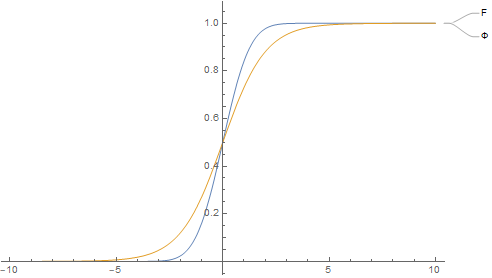
\includegraphics[width=0.6\textwidth]{imagenes3/logit.png}
\end{figure}

\section{Riesgo, oportunidad, riesgo relativo y odds ratio}
Iluestremos estos conceptos con un ejemplo.
\begin{ejemplo}
    En 1 de cada 200 nacimientos ocurre un parto gemelar. Entonces la probabilidad o \textit{riesgo} de que un embarazo elegido al azar de un parto gemelar es $R_1 = \frac{1}{200}$. Hay un forma de expresar lo mismo en términos de apuestas, de 200 partos, 1 es gemelar y 199 no lo son, es decir $O_1 = \frac{1}{199}$. Nótese que
    \begin{align*}
        O_1 = \frac{R_1}{1-R_1}.
    \end{align*}
    $O_1$ es la \textit{oportunidad}. Se observó que entre 100 muejeres que habían tomado ácido fólico, 3 de cada 200 partos eran gemelar. Ahora,
    \begin{align*}
        R_2 = \frac{3}{200}, \quad O_2 = \frac{3}{197} = \frac{R_2}{1-R_2}.
    \end{align*}
    El aumento del riesgo del embarazo gemeral se puede expresar numéricamente como
    \begin{align*}
        RR :=  \frac{R_2}{R_1} = 3, \quad OR:= \frac{O_2}{O_1} \frac{199 \cdot 3}{197} \approx 3.03.
    \end{align*}
\end{ejemplo}

\begin{defi} \
    \begin{itemize}
        \item El riesgo es la probabilidad de que ocurra un resultado.
        \item La oportunidad es el cociente del número de eventos que producen un resultado entre el número de eventos que no lo producen.
        \item  El riesgo relativo es el cociente de los riesgos de dos grupos de población.
              \begin{align*}
                  RR = \frac{R_1}{R_2}.
              \end{align*}
        \item La razón de oportunidades es el cociente de las oportunidades de dos grupos de población.
              \begin{align*}
                  OR = \frac{O_1}{O_2}.
              \end{align*}
    \end{itemize}
\end{defi}

\begin{obs}
    Existe una relación entre el riesgo y la oportunidad:
    \begin{align*}
        O = \frac{R}{1-R}.
    \end{align*}
\end{obs}

\section{Regresión logística}
El modelo de regresión logística es:
\begin{align*}
    E(y_i | x_{1i}, \dots, x_{ki}) = p_i = F(\vec{x}_i'\vec{\beta}) = \frac{1}{1 + e^{-\vec{x}_i'\vec{\beta}}}
\end{align*}
Además, hemos visto que:
\begin{align*}
    \vec{x}_i'\vec{\beta} = \log\left(\frac{p_i}{1-p_i}\right)
\end{align*}
Luego queremos estimar:
\begin{align*}
    \widehat{p}_i = \frac{1}{1 + e^{-\vec{x}_i'\widehat{\vec{\beta}}}}
\end{align*}
Para encontrar los estimadores $\widehat{\beta}_i$ usamos el método de máxima verosimilitud.
Calculamos la función de verosimilitud:
\begin{align*}
    L(\beta_0, \dots, \beta_k) = \prod_{i=1}^n p_i^{y_i}(1-p_i)^{1-y_i}
\end{align*}
Tomamos logaritmos en ambos miembros de la igualdad:
\begin{align*}
    \log L(\beta_0, \dots, \beta_k) & = \sum_{i=1}^n y_i\log(p_i) + \sum_{i=1}^n (1-y_i)\log(1-p_i)                                                                                                                                                              \\
                                    & = \sum_{i=1}^n y_i\log\left(\frac{p_i}{1-p_i}\right) + \sum_{i=1}^n \log(1-p_i) = \sum_{i=1}^n y_i \vec{x}_i'\vec{\beta} + \sum_{i=1}^n \log\left(\frac{e^{-\vec{x}_i'\vec{\beta}}}{1 + e^{-\vec{x}_i'\vec{\beta}}}\right) \\
                                    & = \sum_{i=1}^n y_i \vec{x}_i'\vec{\beta} + \sum_{i=1}^n \log\left(\frac{1}{e^{\vec{x}_i'\vec{\beta}} + 1}\right) = \sum_{i=1}^n y_i \vec{x}_i'\vec{\beta} - \sum_{i=1}^n \log(1 + e^{\vec{x}_i'\vec{\beta}})
\end{align*}
Así que, derivando tenemos que:
\begin{align*}
    \frac{\partial \log L}{\partial \vec{\beta}} = \sum_{i=1}^n y_i\vec{x}_i - \sum_{i=1}^n \frac{\vec{x}_i e^{\vec{x}_i'\vec{\beta}}}{1 + e^{\vec{x}_i'\vec{\beta}}}
\end{align*}
Para hallar los $\widehat{\beta}_i$ hay que resolver el sistema $\frac{\partial \log L}{\partial \beta_i} = 0$ para todo $i = 0, \dots, k$ numéricamente.

Podemos darles significado a los $\beta_j$. Para ello calculamos la oportunidad:
\begin{align*}
    O(x_{1i}, \dots, x_{ki}) = \frac{p_i}{1-p_i} = \frac{P(Y_i = 1)}{P(Y_i = 0)} = \dfrac{\frac{1}{1+e^{-\vec{x}_i'\vec{\beta}}}}{\frac{e^{-\vec{x}_i'\vec{\beta}}}{1+e^{-\vec{x}_i'\vec{\beta}}}} = e^{\vec{x}_i'\vec{\beta}} = e^{\beta_0 + \beta_1x_{1i} + \dots + \beta_kx_{ki}}
\end{align*}
Calculamos ahora la razón de oportunidades cuando aumenta $x_{ji}$ en una unidad:
\begin{align*}
    OR_j = \frac{O(x_{1i}, \dots, x_{ji}+1, \dots, x_{ki})}{O(x_{1i}, \dots, x_{ji}, \dots, x_{ki})} = e^{\beta_j}
\end{align*}
Así que $e^{\beta_j}$ es lo que varía la oportunidad cuando aumenta la componente $j$-ésima en una unidad. Luego $OR_j$ determina si las variable $j$-ésima es significativa.